\chapter{Design af brugergrænsefladen}
\label{Design_G}
Dette kapitel beskriver brugergrænsefladen samt de beslutninger, som ligger bag. Alle vores papermockups og endelige skærmbilleder findes i appendix \ref{App_GUI}.

\section{Workflows}
\label{Design_G_wf}
\label{Design_G_Development}
\begin{figure}[h!]
  \centering
    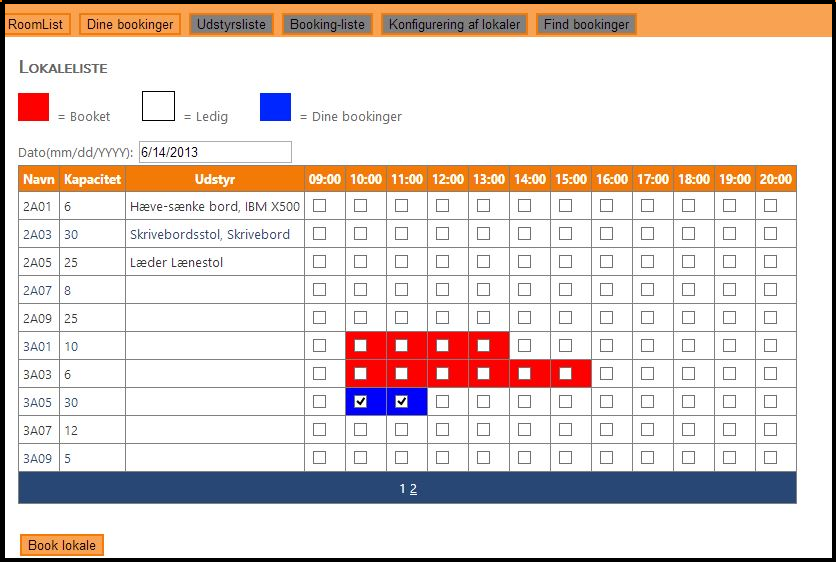
\includegraphics[width=0.85\textwidth]{Appendix/GUI-Prototype/DigitalMockup/GridEksempel}
  \caption{Skærmbilledet til booking af lokaler}
\label{Design_G_wf_FinalGrid}
\end{figure}

Figur \ref{Design_G_wf_FinalGrid} viser startskærmen til vores system. Det er en liste over de lokaler, som kan bookes i systemet. Kolonnerne viser i hvilke tidsrum et bestemt lokale er til rådighed. Hvis brugeren prøver at navigere til en anden del af systemet, vil han blive bedt om at logge ind. Øverst i skærmbilledet vil der altid være en menubar, som giver mulighed for at navigere rundt i systemet.

\textbf{Book lokale}
\\Hvis en bruger vil booke et lokale, skal han vælge et tidsrum i lokalelisten ved markerer de tilsvarende checkbokse. Herefter skal han trykke "Book lokale". Hvis brugeren ikke er logget ind, vil han få vist login-skærmen, hvor han skal logge ind. Han vil herefter få vist listen over sine bookinger (figur \ref{Design_G_wf_YourBookings_Final}), hvor den nye booking vil ligge. Brugeren er nu færdig med at booke lokalet og kan logge af. 

\begin{figure}[h!]
  \centering
    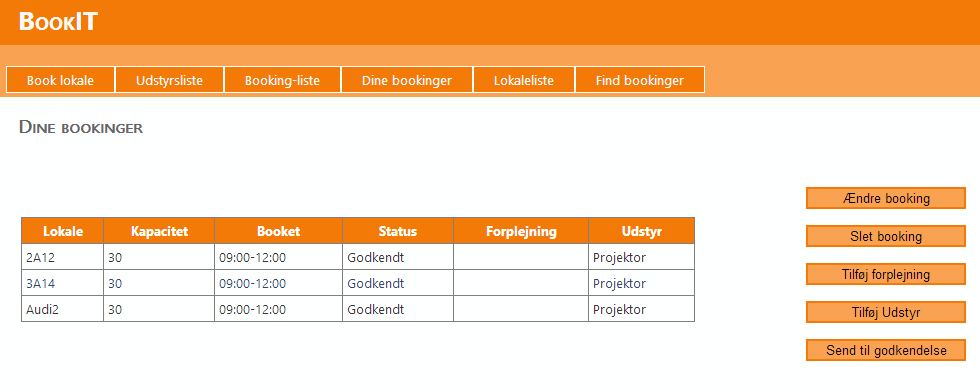
\includegraphics[width=0.9\textwidth]{Appendix/GUI-Prototype/DigitalMockup/DineBookinger}
  \caption{Skærmbilledet til visning brugerens bookinger}
\label{Design_G_wf_YourBookings_Final}
\end{figure}

\textbf{Bestilling af forplejning}
\begin{figure}[h!]
  \centering
    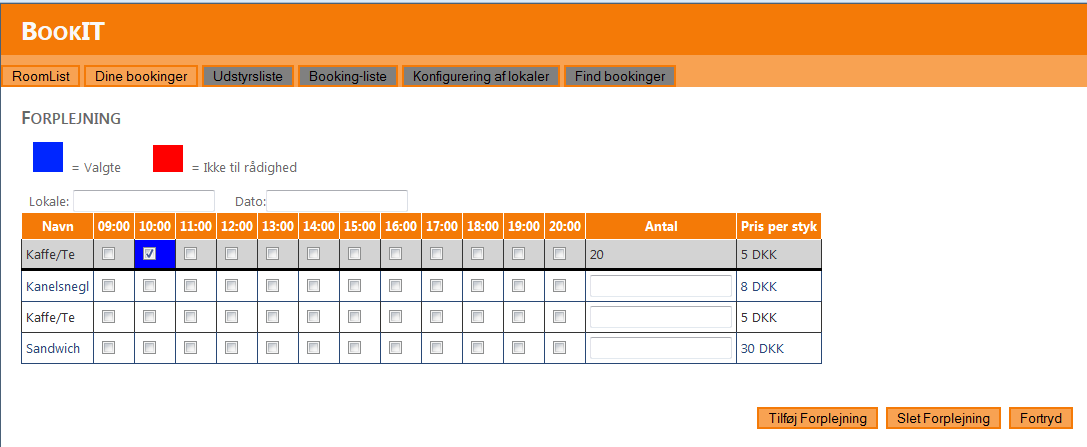
\includegraphics[width=0.9\textwidth]{Appendix/GUI-Prototype/DigitalMockup/Forplejning}
  \caption{Skærmbilledet til bestilling af forplejning}
\label{Design_G_wf_Forplejning_Final}
\end{figure} 
\\Hvis en bruger ønsker at bestille forplejning, skal han trykke på "Dine Bookinger" i menubaren. Hvis han ikke er logget ind, vil han blive bedt om at gøre dette. I listen over sine bookinger skal brugeren vælge den booking, han vil tilføje forplejning til, og trykke på knappen "Tilføj Forplejning". Han bliver nu vist skærmbilledet "Forplejning" (figur \ref{Design_G_wf_Forplejning_Final}), hvor han skal finde forplejningstypen, han ønsker at bestille. 
\\Han skal så udfylde antals feltet samt vælge et enkelt tidspunkt for levering af forplejningen. Han færdiggør bestillingen ved at trykke "Tilføj Forplejning". Brugeren er nu færdig og kan logge ud af systemet. Alternativt kan han trykke "Fortryd" for vende tilbage til skærmbilledet "Dine Bookinger".

\textbf{Administrering af bruger-bookinger}
\begin{figure}[h!]
  \centering
    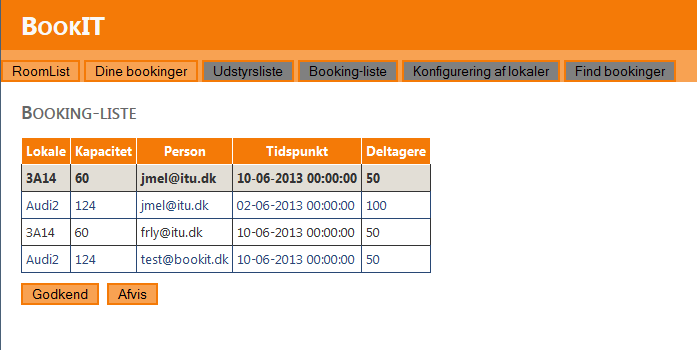
\includegraphics[width=0.8\textwidth]{Appendix/GUI-Prototype/DigitalMockup/BookingListe}
  \caption{Skærmbilledet til godkendelse og afvisning af bookinger}
\label{Design_G_Development_BookingListe_Final}
\end{figure} 
\\Hvis en administrator vil godkende en brugers booking\footnote{Bookinger oprettet af ikke-administratorer skal godkendes af en administrator.}, skal han gå til "Booking-Liste" gennem menubaren. Her vil han blive vist en liste af bookinger, som venter på godkendelse (figur \ref{Design_G_Development_BookingListe_Final}). Han skal her markerer en booking i listen og enten trykke på "Godkend" eller "Afvis". Bookingen vil forsvinde fra listen og administratoren er nu færdig.

\textbf{Administrering af udstyr}
\begin{figure}[h!]
  \centering
    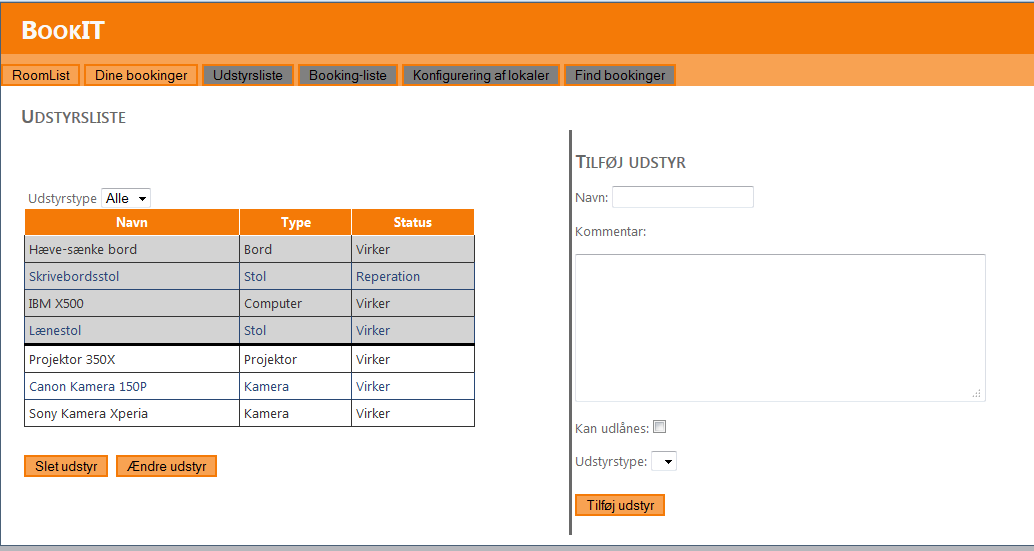
\includegraphics[width=0.9\textwidth]{Appendix/GUI-Prototype/DigitalMockup/UdstyrsListe}
  \caption{Skærmbilledet af receptionistens liste over udstyr i systemet.}
\label{Design_G_Development_UdstyrsListe_Final}
\end{figure} 
\\Hvis en administrator vil redigere i listen over udstyr i systemet, skal han navigere til udstyrslisten gennem menubaren. Han vil nu blive vist listen over udstyr (figur \ref{Design_G_Development_UdstyrsListe_Final}). 
\\Hvis han vil tilføje nyt udstyr til systemet, skal han udfylde felterne i højre side og trykke "Tilføj udstyr". Dette vil oprette udstyret i systemet og vise det i listen til venstre. Han er nu færdig med at tilføjet udstyret og kan logge af.
\\Alternativt kan han slette udstyr eller inventar fra listen i venstre side ved at vælge udstyret/inventaret og trykke på "Slet udstyr". Udstyret/inventaret vil forsvinde fra listen og han er nu færdig med at slette udstyret.

\textbf{Administrering af lokaler}
\begin{figure}[h!]
  \centering
    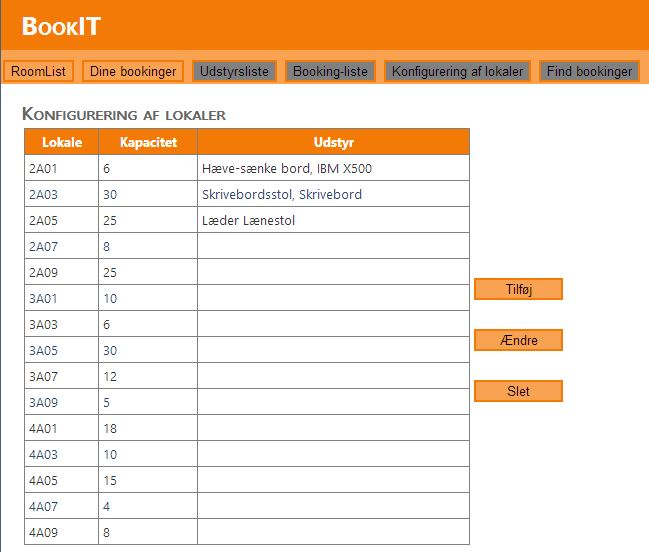
\includegraphics[width=0.9\textwidth]{Appendix/GUI-Prototype/DigitalMockup/LokaleListe}
  \caption{Skærmbilledet af receptionistens liste over udstyr i systemet.}
\label{Design_G_Development_LokaleListe_Final}
\end{figure}
\begin{figure}[h!]
  \centering
    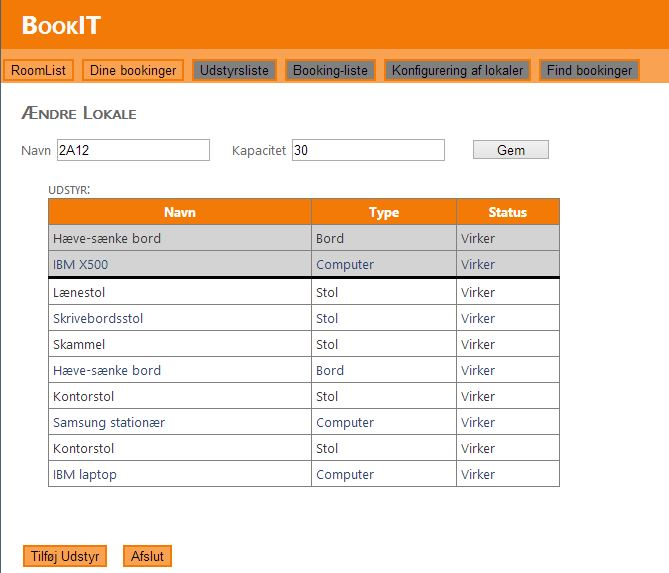
\includegraphics[width=0.8\textwidth]{Appendix/GUI-Prototype/DigitalMockup/AendreLokale}
  \caption{Skærmbilledet til ændring af lokale.}
\label{Design_G_Development_AendreLokale_Final}
\end{figure} 
\\Hvis en administrator vil ændre et lokale, skal han navigere til "Konfigurering af lokaler" i menubaren. Han vil nu blive vist en liste over lokaler i systemet (figur \ref{Design_G_Development_LokaleListe_Final}). Her er der mulighed for at tilføje/slette lokaler samt ændre i eksisterende lokaler. Administratoren kan redigere et lokale ved at vælge det i listen og trykke "Ændre". 
\\Han vil nu blive vist et skærmbillede, som viser lokalets navn, kapacitet samt en liste over inventar. Listen over inventar indeholder både inventar, som er tilføjet det valgte lokale og ledigt inventar.
\\Han kan nu tilføje eller fjerne inventar fra lokalet ved, at han vælger inventaret i listen og trykker på knappen "Tilføj udstyr". Knappen "Tilføj udstyr" skifter tekst, hvis man vælger inventar, som er tilknyttet lokalet. Han er nu færdig og kan navigere væk fra skærmbilledet.

\section{Generelle mål}
\label{Design_G_Goals}
Vores brugergrænseflade er designet ud fra reglerne om design af virtuelle vinduer\cite[s. 169]{SL_UID} samt Ease Of Use principperne\cite[s. 9]{SL_UID}. I forbindelse med dette har vi sat følgende mål for designet:
\begin{itemize}
\item Konsistent brugergrænseflade
\item Få forskellige skærmbilleder
\item Overblik
\item Effektivt
\end{itemize}

\subsection{Konsistent brugergrænseflade}
Skærmbillederne skal have samme grundstruktur. Denne lighed bør gøre det intuitivt at gå fra et skærmbillede til et andet i forbindelse med udførsel af opgaver. Desuden følger det reglen om få vindueskabeloner.

\subsection{Kort vej fra en opgave til en anden}
Brugergrænsefladen skal gøre det hurtigt og nemt for brugeren at komme fra en opgave til en anden. Dette skal gøres ved at have få skærmbilleder involveret i en enkelt task (reglen om få vinduer per opgave).

\subsection{Overblik}
Brugeren skal have mulighed for nemt at danne sig overblik over bookinger, udstyr og forplejning\footnote{Reglen om den nødvendige oversigt af data.}. Derfor skal vi have separate skærmbilleder, som giver overblik over hver type.

\subsection{Effektivt}
Det skal være effektivt at udføre opgaver for brugere, som anvender systemet ofte.

\section{Designets udvikling}
\label{Design_G_du}
